\documentclass[border=10pt]{standalone}
\usepackage{tikz}
\usetikzlibrary{arrows,positioning,shapes.geometric}
\begin{document}
    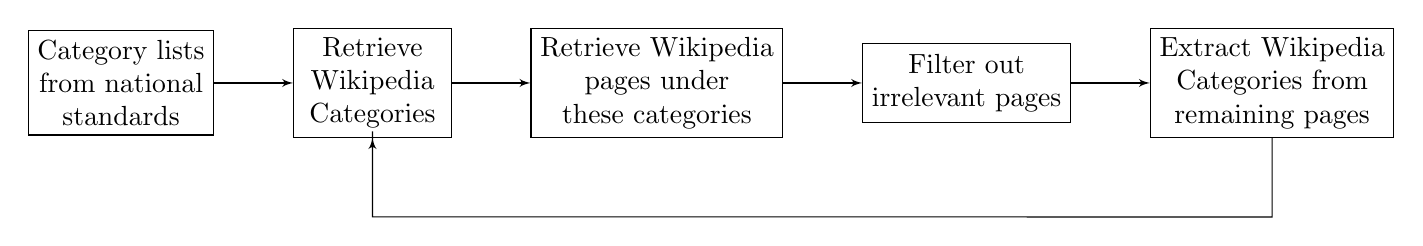
\begin{tikzpicture}[>=latex']
        \tikzset{block/.style= {draw, rectangle, align=center,minimum width=2cm,minimum height=1cm},
        rblock/.style={draw, shape=rectangle,rounded corners=1.5em,align=center,minimum width=2cm,minimum height=1cm},
        input/.style={ % requires library shapes.geometric
        draw,
        trapezium,
        trapezium left angle=60,
        trapezium right angle=120,
        minimum width=2cm,
        align=center,
        minimum height=1cm
    },
        }
        \node [block]  (initcats) {Category lists\\from national\\standards};
        \node [block, right=of initcats] (retcats) {Retrieve\\Wikipedia\\Categories};
        \node [block, right=of retcats] (retpages) {Retrieve Wikipedia\\pages under\\these categories};
        \node [block, right=of retpages] (filter) {Filter out\\irrelevant pages};
        \node [block, right=of filter] (extcats) {Extract Wikipedia\\Categories from\\remaining pages};
        \node [coordinate, below=of extcats] (b1) {};  %% Coordinate on right and middle
        \node [coordinate, below=of retcats] (b2) {};  %% Coordinate on left and middle

%% paths
        \path[draw,->] (initcats) edge (retcats)
                    (retcats) edge (retpages)
                    (retpages) edge (filter)
                    (filter) edge (extcats)
                    (extcats.south) -| (b1) -- (b2) |- (retcats.south)
                    ;
    \end{tikzpicture}
\end{document}

